\documentclass{beamer}
\usepackage[utf8]{inputenc}
\usepackage{amsfonts,amsmath,amssymb}
\usepackage[brazil]{babel}
\usepackage{lipsum}
\usepackage{graphicx}

\usetheme{Frankfurt}
\title{Oficina de \LaTeX}
\author{Nome do mecânico} %autor
\date{18 de outubro de 2016} %data
\institute{IFG}

\begin{document}
\maketitle


\begin{frame}
	\frametitle{Sumário}
	\tableofcontents
\end{frame}
\section{Introdução}

\begin{frame}
\frametitle{Introdução}
\begin{itemize}
\item Apresentações em \LaTeX{} tem caráter muito sério e profissional.
\item Mas o conteúdo não pode deixar a desejar.
\item De nada adianta forma sem conteúdo!
\end{itemize}
\end{frame}

\section{Figuras}
\begin{frame}
\frametitle{Figuras}
\begin{figure}[H]
\centering
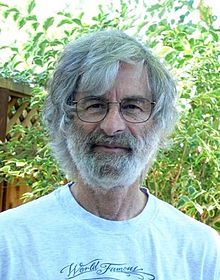
\includegraphics[scale=.7]{figuras/Lamport}
\caption{Leslie Lamport}
\end{figure}
\end{frame}

\section{Conclusão}
\begin{frame}
\frametitle{Fim}
\begin{center}
\Huge{Fim :)}
\end{center}
\end{frame}

\end{document}